\documentclass[a4paper,11pt,notitlepage]{report}

\usepackage[utf8]{inputenc}
\usepackage{amsmath}
\usepackage{listings}
\usepackage[hidelinks]{hyperref}
\usepackage{catoptions}
\usepackage[left=0.8in, right=0.8in, top=0.8in, bottom=0.8in]{geometry}
\usepackage{color}
\usepackage{soul}
\usepackage{float}
\usepackage{framed}
\usepackage[sc]{mathpazo}
\linespread{1.20}         % Palatino needs more leading (space between lines)
\usepackage[T1]{fontenc}
\usepackage{microtype}
\usepackage{enumerate}
\usepackage{courier}
\usepackage{graphicx}
\usepackage{enumitem}
\usepackage{lipsum}
\usepackage{tikz}
\usepackage{caption}
\usepackage{subcaption}
\usepackage{verbatim}
\usetikzlibrary{shapes,arrows}

\graphicspath{ {./Images/} }

\pdfinfo{
  /Title    (Building Serious Games - Design4Health)
  /Author   (Ralf Nieuwenhuizen, David Prihoda, Ismini Psuxoula, Arnold Schutter, Shen Shuheng)
  /Creator  (Ralf Nieuwenhuizen, David Prihoda, Ismini Psuxoula, Arnold Schutter, Shen Shuheng)
  /Producer (Ralf Nieuwenhuizen, David Prihoda, Ismini Psuxoula, Arnold Schutter, Shen Shuheng)
  /Subject  (Building Serious Games)
}

% Settings for hyperref package (e.g. wat \autoref en \nameref moeten doen)
\hypersetup{
  colorlinks  = false,
  linkcolor   = [rgb]{0.1,0.1,0.5},
  citecolor   = [rgb]{0.5,0.1,0.1},
  filecolor   = [rgb]{0.1,0.5,0.5},
  urlcolor    = [rgb]{0.1,0.1,0.7}
}

\newcommand{\todo}[1] {\hl{#1}}
\setlength{\parindent}{0cm}

\begin{document}

% Define block styles
\tikzstyle{block} = [rectangle, draw, fill=white!20, 
    text width=7em, text centered, rounded corners, minimum height=4em]
\tikzstyle{blockSmall} = [rectangle, draw, fill=white!20, 
    text width=4em, text centered, rounded corners, minimum height=3em]
\tikzstyle{line} = [draw, -latex']
		
\begin{center}
\vskip 1cm
{\Huge Design4Health \vskip 2mm}
{\Large Synopsis \& Responsibilities \vskip 1cm}

{\normalsize \textbf{Ralf Nieuwenhuizen ($4080408$) -- \textbf{David Prihoda ($4405951$)} -- \textbf{Ismini Psychoula ($4411285$)} -- \textbf{Arnold Schutter} ($4260724$) -- \textbf{Shuheng Shen ($4298225$)} \vskip 3cm}

\end{center}

%\newpage
%\tableofcontents
%\newpage

\chapter{Team}

Our team consists of $5$ members, all having an own main responsibility. 

\section{Responsibilities}

\begin{itemize}
	\item Ralf Nieuwenhuizen: Communication
	\item David Prihoda: Lead Artist
	\item Ismini Psychoula: Lead programmer
	\item Arnold Schutter: Lead Game Design
	\item Shuheng Shen: Lead Testing
\end{itemize}

\subsection{Communication}
The communicator is responsible for the timely communication with external parties and the teacher including weekly updates. 

\subsection{Lead Artist}
The lead artist is responsible for gameplay and graphics. Gameplay (fun) should continuously be checked and the graphics should be made according to a graphical design plan. The lead artist is responsible for this plan and prioritizing tasks.

\subsection{Lead Programmer}
The lead programmer is responsible for keeping the overview of the software (architecture) and for quality. The lead programmer prioritizes the milestones for the software and checks for the quality and coherence. When deliverables are not satisfactory, the lead programmer is allowed to let deliverables be rectified.

\subsection{Lead Game Design}
The lead game designer is responsible for the overall planning and the coherence between the software and the game design. 

\subsection{Lead Testing}
The lead tester is responsible for weekly testing the deliverables for appearance, errors/bugs, gameplay quality and coherence. The Lead Tester prioritizes the tasks to be improved together with the Lead Programmer. 

\section{Planning}

\subsection{Meetings}
Our weekly meetings are at:
\begin{itemize}
	\item Monday $08.45$ - $10.30$
	\item Tuesday $12.30$ - $16.30$
	\item Thursday $13.45$ - $15.30$
	\item Friday $13.45$ - $16.30$
\end{itemize}

\subsection{Schedules}

\begin{figure}[H]
	\centering
		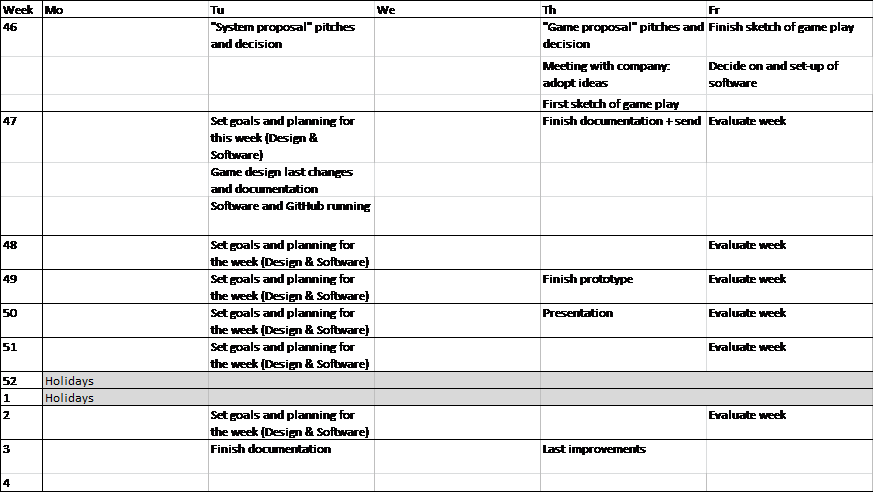
\includegraphics[width=1.00\textwidth]{Images/PlanningSmall.png}
	\caption{Global planning of the project}
	\label{fig:Planning}
\end{figure}

\begin{figure}[H]
	\centering
		
\includegraphics[width=1.00\textwidth]{Images/Todolist.png}
	\caption{Global todo list of the project}
	\label{fig:Todolist}
\end{figure}

\chapter{Game design}
The official game description does not contain specific requirements. The purpose of the game is to motivate or help people to do their exercises, possibly for tasks provided by a physiotherapist. \\
\\
The first concept of design is an engaging game for which the user needs to gather more points to get better in the game. The points can be gathered by doing the exercises according to the training scheme, possibly provided by a physiotherapist. Every successfully completed training day is worth a specific amount of points determined by the physiotherapist. While the user is doing the exercises properly every day, the points are multiplied so each training day will be worth more points over time, we call this a combo. Skipping a training day will stop the combo. \\
\\
To control the user for doing the exercises properly, training data should be uploaded after completing the daily training. When the data is uploaded to the system, the user will receive the points immediately. These points should motivate the user to continue doing the exercises. \\
\\
The data can be checked by a supervisor like the physiotherapist at any moment once in a while to check for correct execution of the exercise. The required data type differs per type of exercise. For specific exercises provided by the physiotherapist the user could make a video of the execution of the exercises. GPS-data would be more useful when the exercises are running, cycling or walking. \\
\\
Several engaging games should be available in a game platform, specific for different age categories and gender, from which a user can pick one game. The game platform will work independently so new games can be plugged in into the system. The games should however facilitate the input of gathered points directly in the game. \\
\\
The construct of the system is shown in \ref{fig:gamedesignscheme}. 

\begin{figure}[H]
	\centering
		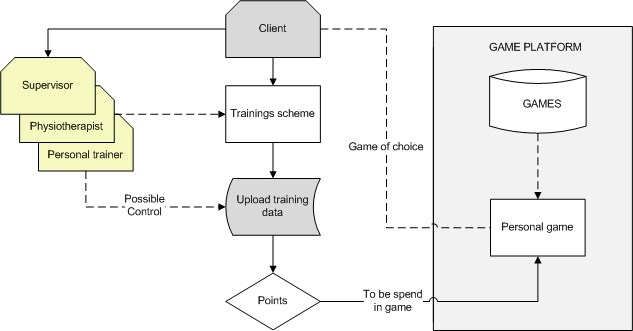
\includegraphics[width=0.80\textwidth]{Images/gamedesignscheme.jpg}
	\caption{Scheme of the game design}
	\label{fig:gamedesignscheme}
\end{figure}



%\bibliography{synopsis}
%\bibliographystyle{plain}

\end{document}
